% Created 2024-01-13 Sat 03:09
% Intended LaTeX compiler: xelatex
\documentclass[11pt]{article}
\usepackage{graphicx}
\usepackage{longtable}
\usepackage{wrapfig}
\usepackage{rotating}
\usepackage[normalem]{ulem}
\usepackage{amsmath}
\usepackage{amssymb}
\usepackage{capt-of}
\usepackage{hyperref}
\usepackage{minted}
\usepackage[margin=2cm]{geometry}
\input{~/.doom.d/fancyLatexTemplate.tex}
\author{Spyridon Baltsas - AEM: 10443}
\date{}
\title{Parallel and Distributed Systems - Kth Select Report}
\hypersetup{
 pdfauthor={Spyridon Baltsas - AEM: 10443},
 pdftitle={Parallel and Distributed Systems - Kth Select Report},
 pdfkeywords={},
 pdfsubject={},
 pdfcreator={Emacs 28.2 (Org mode 9.6.1)}, 
 pdflang={English}}
\begin{document}

\maketitle

\section{Summary}
\label{sec:orgd347248}
This report is about my proposed solution for Kth Select problem. To be more specific, here are briefly presented and explained the algorithms I have implemented for my approach for both single process and multiple processes with distributed memory use cases. Additionally, the efficiency of MPI algorithm against various large datasets will be examined for different amount of processes, and MPI's effectiveness itself when it comes to distributing processes among several compute instances.
\section{Algorithm}
\label{sec:org3cef1c7}
\subsection{The problem}
\label{sec:org1c9d8f8}
The problem is stated like this: ``In a vector of unsorted elements, find which element would be in the \$k\$-th position if the vector was sorted in ascending order''.
\subsection{Approach}
\label{sec:org7ec71b5}
\subsubsection{Sequential}
\label{sec:org80cc15f}
The most effective algorithm to address this problem is QuickSelect. QuickSelect is very similar to QuickSort. A pivot element is selected from the array, and after using the \texttt{partition} function. The Lomuto's partitioning scheme was selected for the sake of simplicity. As a result, array is splitted in two sub-arrays;
\begin{itemize}
\item A sub-array containing elements which are smaller or equal to the pivot.
\item A sub-array containing elements larger than pivot.
\end{itemize}
Here is the point where QuickSelect differs from QuickSort. Instead of recursing on both subarrays, we recurse on the subarray where the k-th is included. For example, if k is larger than the position of pivot, then we recurse to the sub-array containing the elements larger than pivot. Finally, the algorithm stops when k is equal to the position of pivot element. In that case, the problem is solved, we found the k-th smallest element.

It can be proven that the average time complexity is linear (\(\mathcal{O}(n)\)), and square (\(\mathcal{O}(n^{2})\)) in the worst case where the array is already sorted.
\subsubsection{Parallel / Distributed Memory}
\label{sec:org9c77196}
Since QuickSelect appears to be that fast when a single process is used, I attempted to create an implementation for distributed systems using the MPI library. In such a distributed memory environment, MPI is currently the only way to go. As a result, since shared memory between processes is completely absent, the task of implementing the quickselect algorithm in such a stable way may get very challenging for the following reasons;
\begin{itemize}
\item Starvation of root process. The process who controls the other processes (also known as the root process) by advertising the pivot, may run out of elements and therefore rely on the elements of the other processes to find the pivot element that should be picked correctly. As a result, there will be an overhead of processes communicating with each other, especially when processes are on different computers.
\item Some processes may have all of the elements in their subarrays either larger or smaller as pivot, and because of that they may be not able to contribute to speeding up the search for the k-th element any further.
\item Recursive nature of algorithm itself. There may be few extreme cases, sometimes very hard to predict, on which algorithm may fail to provide an answer, where either the answer will be incorrect or get stuck in an infinite loop. In addition, a recursive algorithm may not be able to get parallelized as efficiently as an imperative one could be.
\end{itemize}
\uline{DISCLAIMER:} As the README of my repository states, the MPI version may get stuck in an infinite loop for a few cases. The reason is currently unknown. In case it happens, please try changing the number of processes, since it has been observed that fixes the issue most of the times.

Taking the above points into consideration the QuickSelect was modified. The behavior of algorithm changes slightly whether process is the controlling one or not. The logic can be summed up in the following steps;
\begin{enumerate}
\item Root process selects a pivot. If it has elements left, the last element of array is selected. Otherwise it is depleted, the smallest element of the rest of processes is selected as the pivot. The root process announces the pivot to the rest of processes.
\item All processes split their arrays again in 2 subarrays with the same partitioning scheme as the sequential, one containing elements less or equal to pivot (left sub-array), and one containing elements larger than pivot (right sub-array).
\item The amount of elements that is smaller than pivot and the amount of elements that are equal to that are calculated, in order the global position (the position of pivot in the sequential QuickSelect) of pivot to be found. Let \(p\) be the global pivot position and \(d\) be the amount of elements equal to pivot. If \(k\) belongs to the \([p, p+d)\) set, then the value of k-th element is found. The algorithm stops.
\item Otherwise, the following actions are taken;
\begin{enumerate}
\item If \(k < p\);
\begin{enumerate}
\item If process is the root and all elements are larger than pivot, process is depleted. Otherwise, find the position of the last element smaller than pivot and recurse into the resulting sub-array.
\item If the process is not the root, and the global position is out of the bounds of the current array, it is considered depleted and recurses into the same array (idles). Otherwise, if the element at the global position is equal to pivot, recurse on the left sub-array, excluding the element equal to pivot. If less than pivot, then again recurse on the left sub-array but contain the element as well.
\end{enumerate}
\item If \(k > p\), then similarly;
\begin{enumerate}
\item If process is the root and all elements except pivot are less than it, process is depleted. Otherwise, find the position of the last element larger than pivot and recurse into the resulting sub-array.
\item If the process is not the root, and the global position is out of the bounds of the current array, it is considered depleted and recurses into the same array (idles). Otherwise, if the element at the global position is equal to pivot, recurse on the right sub-array, excluding the element equal to pivot. If larger than pivot, then again recurse on the right sub-array but contain the element as well.
\end{enumerate}
\end{enumerate}
\end{enumerate}
\pagebreak
\section{Test Specifications}
\label{sec:orge906da4}
\subsection{System Specifications}
\label{sec:orgcc98fa9}
\subsubsection{Sequential}
\label{sec:orgbb0a366}
\subsubsection{Parallel / Distributed}
\label{sec:org543559e}
\subsection{Test Dataset Specifications}
\label{sec:org1d72e11}
\begin{center}
\begin{tabular}{llr}
\hline
Name & File Size & 32-bit Integer Count\\[0pt]
\hline
\href{https://dumps.wikimedia.org/other/static\_html\_dumps/current/el/wikipedia-el-html.tar.7z}{Greek Wiki Dump} & 107 MB & 28084359\\[0pt]
\href{https://developer.download.nvidia.com/compute/cuda/12.0.0/local\_installers/cuda\_12.0.0\_525.60.13\_linux.run}{NVIDIA CUDA 12 Linux Runfile} & 3.8 GB & 1030846977\\[0pt]
\hline
\end{tabular}
\end{center}
\section{Results}
\label{sec:orgb49e4a2}
\subsection{Charts}
\label{sec:orgdbf1a55}
\subsubsection{Greek Wiki Dump}
\label{sec:org60ecbef}
\begin{center}
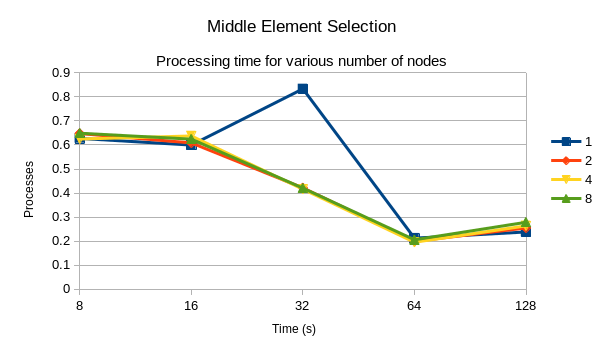
\includegraphics[height=200]{./charts/greek-wiki-dump/processing-time-nodes.png}
\end{center}
\begin{center}
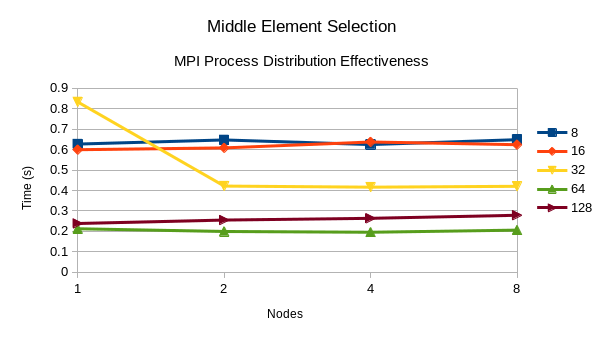
\includegraphics[height=200]{./charts/greek-wiki-dump/process-distribution-effectiveness.png}
\end{center}
\subsubsection{NVIDIA CUDA 12 Linux Runfile}
\label{sec:orgf292482}
\begin{center}
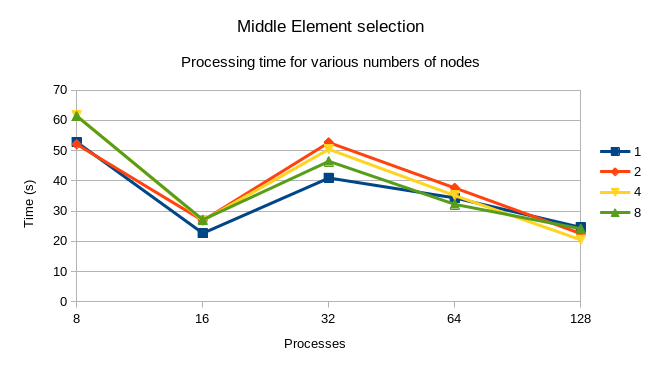
\includegraphics[height=200]{./charts/cuda-12-runfile/processing-time-nodes.png}
\end{center}
\begin{center}
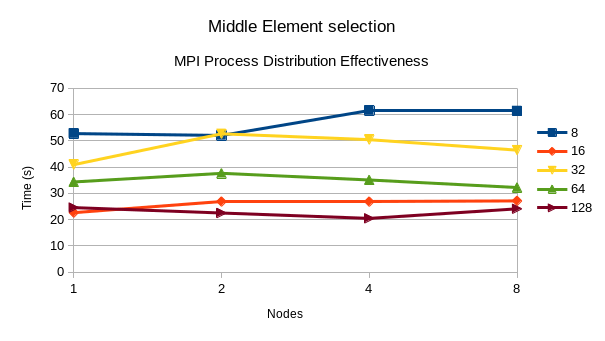
\includegraphics[height=200]{./charts/cuda-12-runfile/process-distribution-effectiveness.png}
\end{center}
\end{document}